%-----------------------------------------------------------------------
% Installation : Subeclipse
% 
%-----------------------------------------------------------------------
%\newpage

%-----------------------------------------------------------------------
\section{Installation du plugin Subclipse dans Eclipse}

Subclipse est un plug-in Eclipse vous permettant d'utiliser Subversion (SVN) directement depuis votre \'editeur pr\'ef\'er\'e.

\begin{itemize}[leftmargin=* ,parsep=0cm,itemsep=0cm,topsep=0cm]

\medskip

\item Etape 1 : Commencer par cliquer dans le menu d’Eclipse sur l'onglet « Help », puis sur « Install New Software ».
\begin{center}
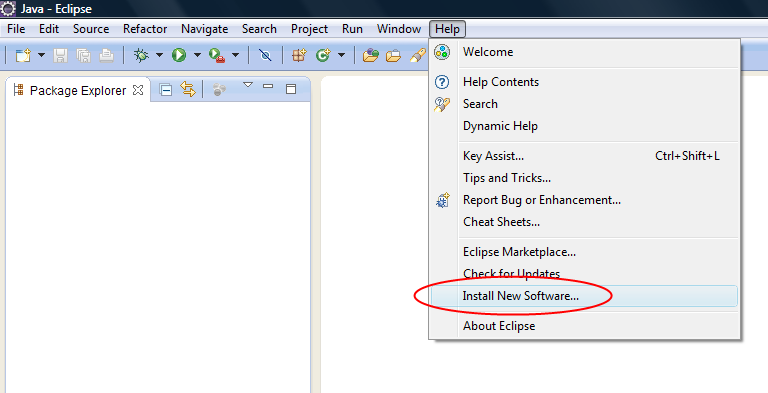
\includegraphics[width=0.4\linewidth]{../../resources/images/guide_installation/pluginInstall.png}
\end{center}

\item Etape 2 : Cliquer sur « Add » afin d’ajouter le site de subeclipse dans la liste des sites de logiciels disponibles
\begin{center}
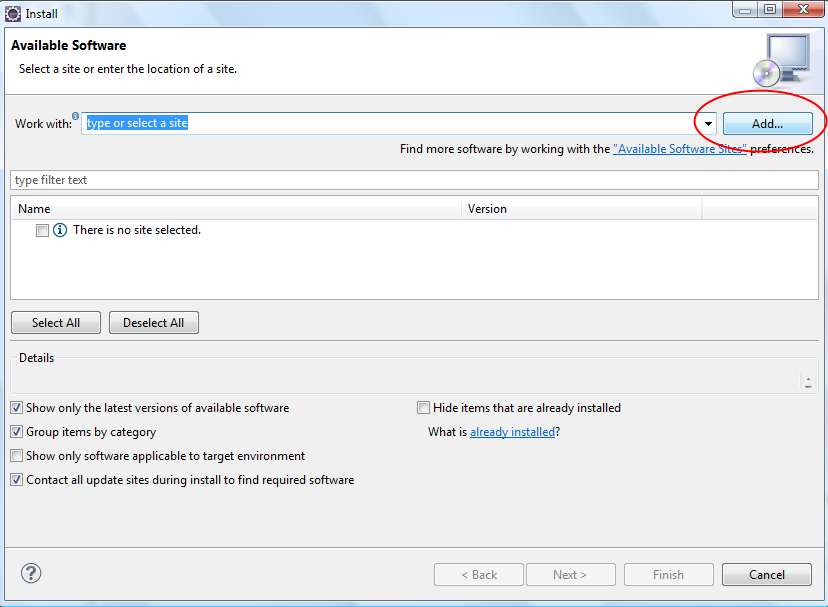
\includegraphics[width=0.4\linewidth]{../../resources/images/guide_installation/pluginNewUrl.png}
\end{center}

\item Etape 3 : Saisir dans la boite de dialogue les informations d\'ecrites ci-dessous puis cliquer sur "OK"\\

\begin{tabular}[!t]{ll}
{\bf Name : }&{Subclispe}\\
{\bf Location : }&{\href{http://subclipse.tigris.org/update_1.8.x}{http://subclipse.tigris.org/update\_1.8.x}}\\
\end{tabular}\\
\smallskip
\begin{center}
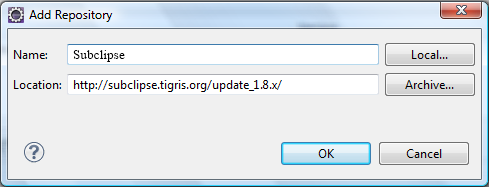
\includegraphics[width=0.4\linewidth]{../../resources/images/guide_installation/subeclipseUrl.png}
\end{center}

\newpage

\item Etape 4 : La boite de dialogue "install" affiche l'ensemble des plugins disponibles. Tout n’est pas utile, mais cocher au moins les packages marqu\'es required ainsi que SVNKit puis cliquer sur "Next".
\begin{center}
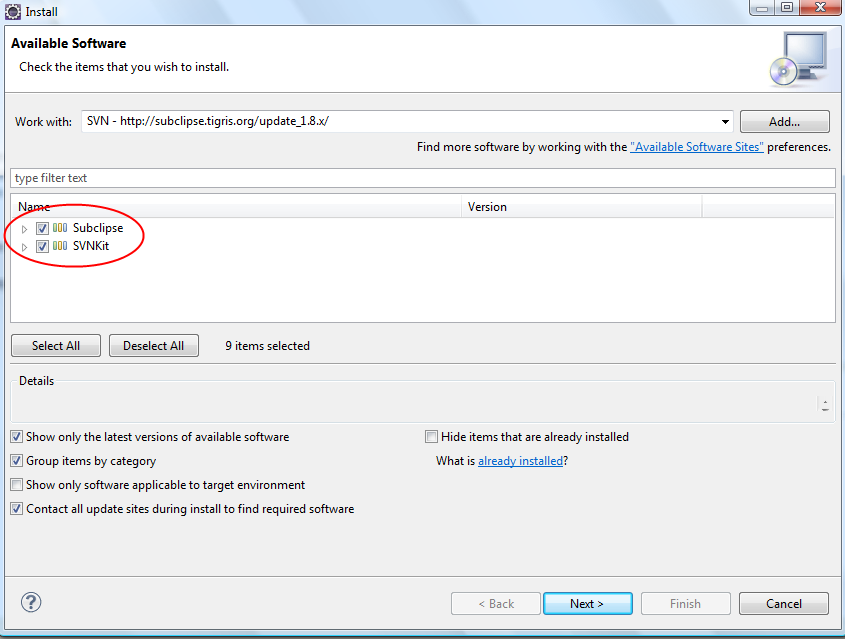
\includegraphics[width=0.4\linewidth]{../../resources/images/guide_installation/subeclipseEtape1.png}
\end{center}

\item Etape 5 : Sur la page "Install Details" cliquer juste sur le bouton "Next"
\begin{center}
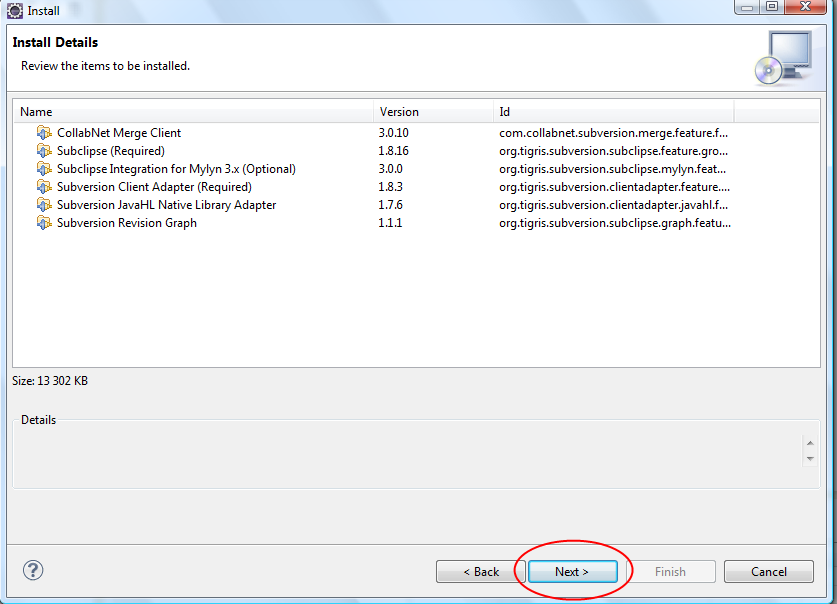
\includegraphics[width=0.4\linewidth]{../../resources/images/guide_installation/subeclipseEtape2.png}
\end{center}

\item Etape 6 : Accepter les termes de la licence de subeclipse sur la page "Review Licences" et cliquer sur "Finish" pour commencer l'installation.
\begin{center}
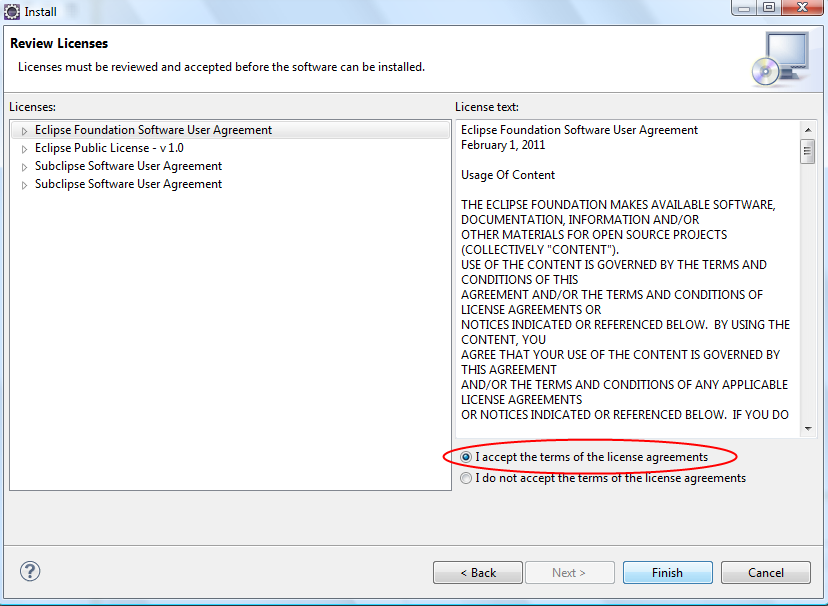
\includegraphics[width=0.4\linewidth]{../../resources/images/guide_installation/subeclipseEtape3.png}
\end{center}

\item Etape 7 : Vous allez recevoir un message d'alerte "Security Warning" parce que les jars de subeclipse ne sont pas sign\'es. Cliquer sur "OK" pour continuer l'installation.
\begin{center}
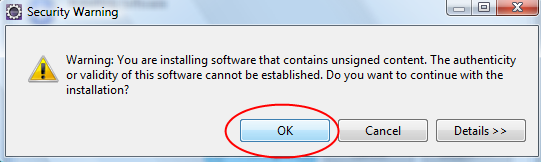
\includegraphics[width=0.4\linewidth]{../../resources/images/guide_installation/pluginNonSigne.png}
\end{center}

\newpage

\item Etape 8 : Une fois l'installation termin\'ee, pr\'ef\'erer "Restart Now" dans la prochaine boite de dialogue. 
\begin{center}
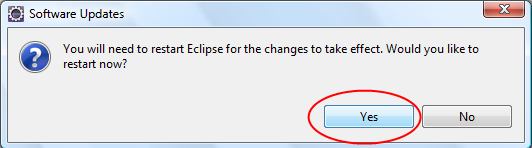
\includegraphics[width=0.4\linewidth]{../../resources/images/guide_installation/pluginRestart.png}
\end{center}
Le plugin subeclipse sera op\'erationnel après le red\'emarrage d'Eclipse.

\bigskip

\item Etape 9 : Une fois le plugin install\'e, configurer dans Eclipse l'interface SVNKit. En effet, celle-ci semble mieux fonctionner que celle par d\'efaut (JavaHL). Pour cela, dans le menu d'Eclipse Window/Preferences/Team/SVN, s\'electionner l’interface SVN "SVNKit".
\begin{center}
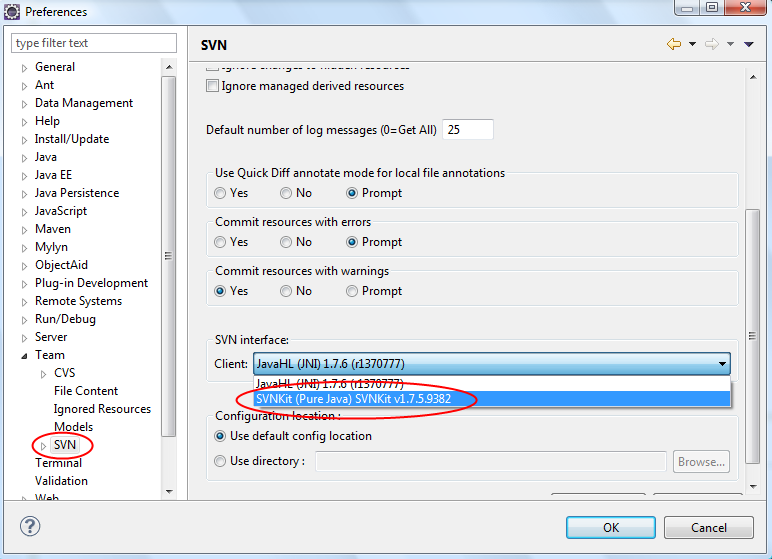
\includegraphics[width=0.4\linewidth]{../../resources/images/guide_installation/subeclipseInterface.png}
\end{center}


\end{itemize}